\chapter{Project Plan}

\section{Project Estimates}
The project was planned using an iterative software development approach. The work was divided into requirement analysis, literature survey, design, implementation, integration, testing, and documentation.

\begin{enumerate}
\item \textbf{Requirement Gathering}: The team studied the need for image geolocation, scene explanation, risk triage, user-confirmed reporting, and audit logging.
\item \textbf{Analysis}: Functional requirements, non-functional requirements, user roles, model constraints, and safety requirements were identified.
\item \textbf{Design}: The team designed the system architecture, data model, API flow, UI flow, and risk-to-action policy.
\item \textbf{Implementation}: The backend, frontend, database schema, model integration, action handlers, and incident logging were implemented.
\item \textbf{Testing}: Normal landmark images, hazardous images, ambiguous cases, learn-more actions, and report flows were tested.
\item \textbf{Documentation}: The final report, research paper, diagrams, results, limitations, and future scope were prepared.
\end{enumerate}

\subsection{Reconciled Estimates}
\subsubsection{Cost Estimate}
The project uses open-source development tools and academic infrastructure. The main cost components are internet usage, development machines, optional API usage, and documentation/printing. Since the prototype runs locally and uses SQLite, infrastructure cost is minimal.

\begin{table}[H]
\centering
\caption{Cost Estimate}
\begin{tabularx}{\textwidth}{|c|X|c|}
\hline
\textbf{Sr. No.} & \textbf{Resource} & \textbf{Estimated Cost} \\ \hline
1 & Development laptops and college laboratory facilities & Existing resources \\ \hline
2 & Open-source software tools & No direct cost \\ \hline
3 & Internet and API access for model testing & Variable / demo usage \\ \hline
4 & Report printing and binding & As per college requirement \\ \hline
\end{tabularx}
\end{table}

\subsubsection{Time Estimates}
\begin{table}[H]
\centering
\caption{Time Estimate}
\begin{tabularx}{\textwidth}{|c|X|c|}
\hline
\textbf{Sr. No.} & \textbf{Activity} & \textbf{Duration} \\ \hline
1 & Requirement analysis and literature survey & 3 weeks \\ \hline
2 & System design and database design & 2 weeks \\ \hline
3 & Backend and model integration & 4 weeks \\ \hline
4 & Frontend development and action workflow & 4 weeks \\ \hline
5 & Testing, metrics, and report preparation & 3 weeks \\ \hline
\end{tabularx}
\end{table}

\subsection{Project Resources}
\begin{itemize}
\item \textbf{People}: Four student developers, internal guide, project coordinator, and reviewers.
\item \textbf{Hardware}: Development laptops with internet connection.
\item \textbf{Software}: Python, Flask, SQLite, React, Vite, TypeScript, Tailwind CSS, Gemini Vision API, Wikipedia package, LaTeX.
\item \textbf{Tools}: VS Code, Git, browser developer tools, draw.io/diagram tools, pdflatex.
\end{itemize}

\section{Risk Management w.r.t. NP Hard Analysis}
The project is not an NP-hard optimization problem in the classical computational sense. However, it contains uncertainty and risk because visual scene interpretation, geolocation, and hazard detection are open-ended AI tasks. Risk management therefore focuses on model uncertainty, fallback behavior, API failure, privacy, and false alerts.

\subsection{Risk Identification}
\begin{itemize}
\item Model returns invalid or incomplete JSON.
\item Model produces incorrect location or risk level.
\item Hazard keyword fallback creates false alerts.
\item API key or network failure prevents model inference.
\item User reports an incident without proper context.
\item Raw image storage may create privacy concerns.
\end{itemize}

\subsection{Risk Analysis}
\begin{table}[H]
\begin{center}
\caption{Risk Table}
\label{tab:risk}
\def\arraystretch{1.4}
\begin{tabularx}{\textwidth}{|c|X|c|c|c|c|}
\hline
\multirow{2}{*}{ID} & \multirow{2}{*}{Risk Description} & \multirow{2}{*}{Probability} & \multicolumn{3}{|c|}{Impact} \\ \cline{4-6}
 & & & Schedule & Quality & Overall \\ \hline
1 & Invalid model output or parsing failure & Medium & Low & High & High \\ \hline
2 & Incorrect risk classification & Medium & Low & High & High \\ \hline
3 & Gemini API unavailable or key missing & Low & Medium & Medium & Medium \\ \hline
4 & False incident report by user & Low & Low & High & High \\ \hline
5 & Privacy concern due to image handling & Low & Low & High & High \\ \hline
\end{tabularx}
\end{center}
\end{table}

\subsection{Overview of Risk Mitigation, Monitoring, Management}
\begin{table}[H]
\centering
\caption{Risk Mitigation Plan}
\def\arraystretch{1.4}
\begin{tabularx}{\textwidth}{|c|X|X|}
\hline
\textbf{Risk ID} & \textbf{Mitigation Strategy} & \textbf{Monitoring Method} \\ \hline
1 & JSON extraction, one repair pass, and safe fallback response & Check model output logs \\ \hline
2 & Deterministic confidence thresholds and hazard policy rules & Review risk distribution and sample outputs \\ \hline
3 & Clear backend error handling and fallback messages & Monitor API response errors \\ \hline
4 & Require explicit user confirmation before incident creation & Review incident table \\ \hline
5 & Store image hash instead of raw image by default & Inspect message records and configuration \\ \hline
\end{tabularx}
\end{table}

\section{Project Schedule}
\subsection{Project Task Set}
\begin{itemize}
\item Task 1: Domain finalization and literature survey.
\item Task 2: Requirement analysis and SRS preparation.
\item Task 3: UI, API, database, and policy design.
\item Task 4: Backend implementation and Gemini integration.
\item Task 5: Frontend implementation and action buttons.
\item Task 6: Testing with normal, hazardous, and ambiguous images.
\item Task 7: Metrics analysis, report writing, and paper preparation.
\end{itemize}

\subsection{Task Network}
The task network follows a dependency chain: literature survey and requirements lead to architecture design; architecture design leads to backend and frontend implementation; implementation leads to testing; testing leads to result analysis and documentation.

\subsection{Timeline Chart}
\begin{table}[H]
\centering
\caption{Timeline Chart}
\def\arraystretch{1.3}
\begin{tabularx}{\textwidth}{|c|X|l|l|}
\hline
\textbf{Sr. No.} & \textbf{Task Name} & \textbf{Start Month} & \textbf{End Month} \\ \hline
1 & Domain study and base paper selection & June 2025 & July 2025 \\ \hline
2 & Requirement analysis and synopsis & August 2025 & September 2025 \\ \hline
3 & System design and diagrams & September 2025 & October 2025 \\ \hline
4 & Backend and database implementation & November 2025 & January 2026 \\ \hline
5 & Frontend and action workflow implementation & January 2026 & February 2026 \\ \hline
6 & Testing, evaluation, and report preparation & February 2026 & April 2026 \\ \hline
7 & Final documentation and submission & April 2026 & May 2026 \\ \hline
\end{tabularx}
\end{table}

\section{Team Organization}
\subsection{Team Structure}
The team consists of four student members working under the guidance of the internal guide. Responsibilities were distributed across research, backend, frontend, database, testing, documentation, and presentation.

\begin{figure}[H]
\centering
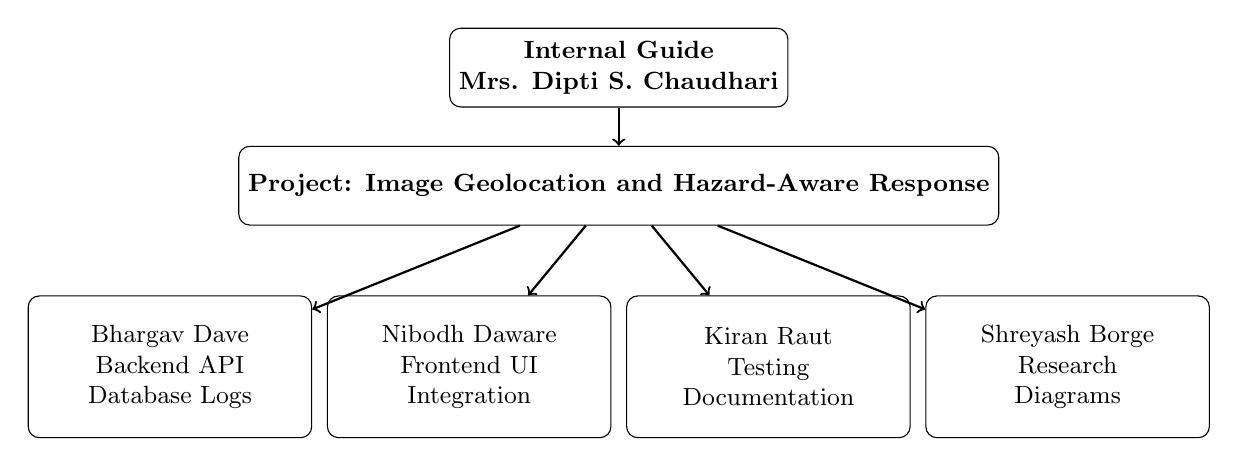
\begin{tikzpicture}[
member/.style={rectangle, draw, rounded corners, minimum width=36mm, minimum height=18mm, align=center, font=\small},
lead/.style={rectangle, draw, rounded corners, minimum width=42mm, minimum height=10mm, align=center, font=\small\bfseries},
flow/.style={->, thick}
]
\node[lead] (guide) at (5.7,1.8) {Internal Guide\\Mrs. Dipti S. Chaudhari};
\node[lead] (project) at (5.7,0.3) {Project: Image Geolocation and Hazard-Aware Response};
\node[member] (bhargav) at (0,-2.0) {Bhargav Dave\\Backend API\\Database Logs};
\node[member] (nibodh) at (3.8,-2.0) {Nibodh Daware\\Frontend UI\\Integration};
\node[member] (kiran) at (7.6,-2.0) {Kiran Raut\\Testing\\Documentation};
\node[member] (shreyash) at (11.4,-2.0) {Shreyash Borge\\Research\\Diagrams};
\draw[flow] (guide) -- (project);
\draw[flow] (project) -- (bhargav);
\draw[flow] (project) -- (nibodh);
\draw[flow] (project) -- (kiran);
\draw[flow] (project) -- (shreyash);
\end{tikzpicture}
\caption{Team structure}
\label{fig:team}
\end{figure}

\subsection{Management Reporting and Communication}
The team followed regular internal discussions, guide reviews, project lab sessions, and milestone-based reporting. Progress was tracked through working demonstrations, report updates, and review feedback.

\begin{table}[H]
\centering
\caption{Management Plan}
\def\arraystretch{1.3}
\begin{tabularx}{\textwidth}{|c|l|X|}
\hline
\textbf{Sr. No.} & \textbf{Month} & \textbf{Description} \\ \hline
1 & June-July & Domain discussion, paper search, and problem finalization. \\ \hline
2 & August-September & Requirement analysis, synopsis, and preliminary design. \\ \hline
3 & October-November & Architecture, database design, and backend planning. \\ \hline
4 & December-February & Implementation of backend, frontend, and action workflow. \\ \hline
5 & March-April & Testing, evaluation, metrics, and report drafting. \\ \hline
6 & May & Final report completion and submission preparation. \\ \hline
\end{tabularx}
\end{table}
